\documentclass[a4paper,10pt]{article}
% Paquetes de la ams
\usepackage{amsmath,amsthm,amssymb,amsfonts}
% Codificacion UTF-8
\usepackage[utf8]{inputenc}
% Tablas e imagenes en espaniol
\usepackage[spanish,es-tabla]{babel}
% Mejores graficos
\usepackage{graphicx}
% tablas mas lindas
\usepackage{booktabs}
% Links a urls
\usepackage{url}
% Linkear referencias en pdfs
\usepackage{hyperref}
% Texto mas lindo para los pie de figura
\usepackage[margin=10pt,font=small,labelfont=bf, labelsep=endash]{caption}

% Citas
\usepackage[backend=biber,style=ieee]{biblatex}
\addbibresource{biblio.bib}

% Codigo
\usepackage{listings}

% Dir tree
\usepackage{dirtree}

% Pagina en blanco cuando ha
\usepackage{emptypage}

\definecolor{A11}{HTML}{B2DF8A}
\definecolor{A12}{HTML}{33A02C}
\definecolor{A23}{HTML}{FDBF6F}
\definecolor{A24}{HTML}{FF7F00}
\definecolor{B15}{HTML}{FB9A99}
\definecolor{B16}{HTML}{E31A1C}
\definecolor{B27}{HTML}{A6CEE3}
\definecolor{B28}{HTML}{1F78B4}

% Ejemplos, observaciones y teorema
\theoremstyle{definition}
\newtheorem{exa}{Ejemplo}[section]
\newtheorem*{obs}{Observación}
\newtheorem{que}{Pregunta}[section]
\newtheorem{dex}{Definicion}[section]

\usepackage{float}
\graphicspath{{./figs/}}

\title{{\large Nivel 0a} \\ Interpretación visual de imágenes satelitales}
\author{Francisco Nemiña \and Marina Compagnucci}
\begin{document}
\maketitle
\titlepage

\section{Introducción}
Existen en la actualidad distintas formas de acceder a productos de origen satelital. Es posible obtener un amplio rango de productos que van desde imágenes en crudo hasta promedios procesados de variables biofísicas.

En los últimos años, además de las formas tradicionales de procesaamiento de imagenes donde un usuario debía descargar un producto para poder manipularlo, comenzaron a apareccer soluciones WEB. Esta nueva forma de procesamiento permite al usuario, independientemente de su nivel de conocimiento, accededr a un amplio abanico de productos. Entre las soluciones existentes se destacan el EarthEngine de Google, el LandsatView de ESRI y el LandView de EOS.

Aunque todas estas soluciones se encuentran disponibles, muchas de ellas sin cargo, existe siempre la necesidad latente de capacitación para un mejor uso de estas herramientas. Pretendemos entonces, en este curso, incorporar los conocimientos básicos de teledetección que permitan a usuarios sin conocimientos previos el acceso a productos satelitales de una forma sencilla y clara.

Para esto, trabajaremos con una aplicación concreta e intentares determinar mediantes el uso de herramientas WEB y con el fin de incorporar conocimientos básicos de teledetección, al superficie incendiada durante el mes de septiembre de 2017 en las cercanias de Carlos Paz, provincia de Cordoba.

\section{Land View}

LandView es un servicio web de la empresa Earth Observing System. Este permite explorar, visualizar y descargar una amplia gama de productos satelitales. El paquete gratuito de la empeza permite visualizar y descargar hasta 10 imagenes por día de sensores que incluyen la serie Landat (1982-actualidad), MODIS (2013-actualidad) y sentinel 2 (2012-actualidad).

Para acceder al servicio de LandView uno debe dirigirse a \href{https://lv.eosda.com} y luego de que termine el tour podra comenzar a utilizarlo. Es recomendable registrar una cuenta gratuita para poder aprovechar más funcionalidades del servicio. Para esto haga click en \emph{Sign in} y registrese utilizando su dirección de correo electronico o acceda con los servicios de Facebook, Google o LinkedIn (Figura \ref{fig:registro})

\begin{figure}[h!]
    \centering
    %\includegraphics{fig:registro.png}
    \caption{}
    \label{fig:registro}
\end{figure}

Una vez registrado, accedera a un mapa  similar al de Google Maps o cualquier SIG (Figura \ref{fig:mapa}). Destacamos en el 3 partes:

\begin{figure}[h!]
    \centering
    %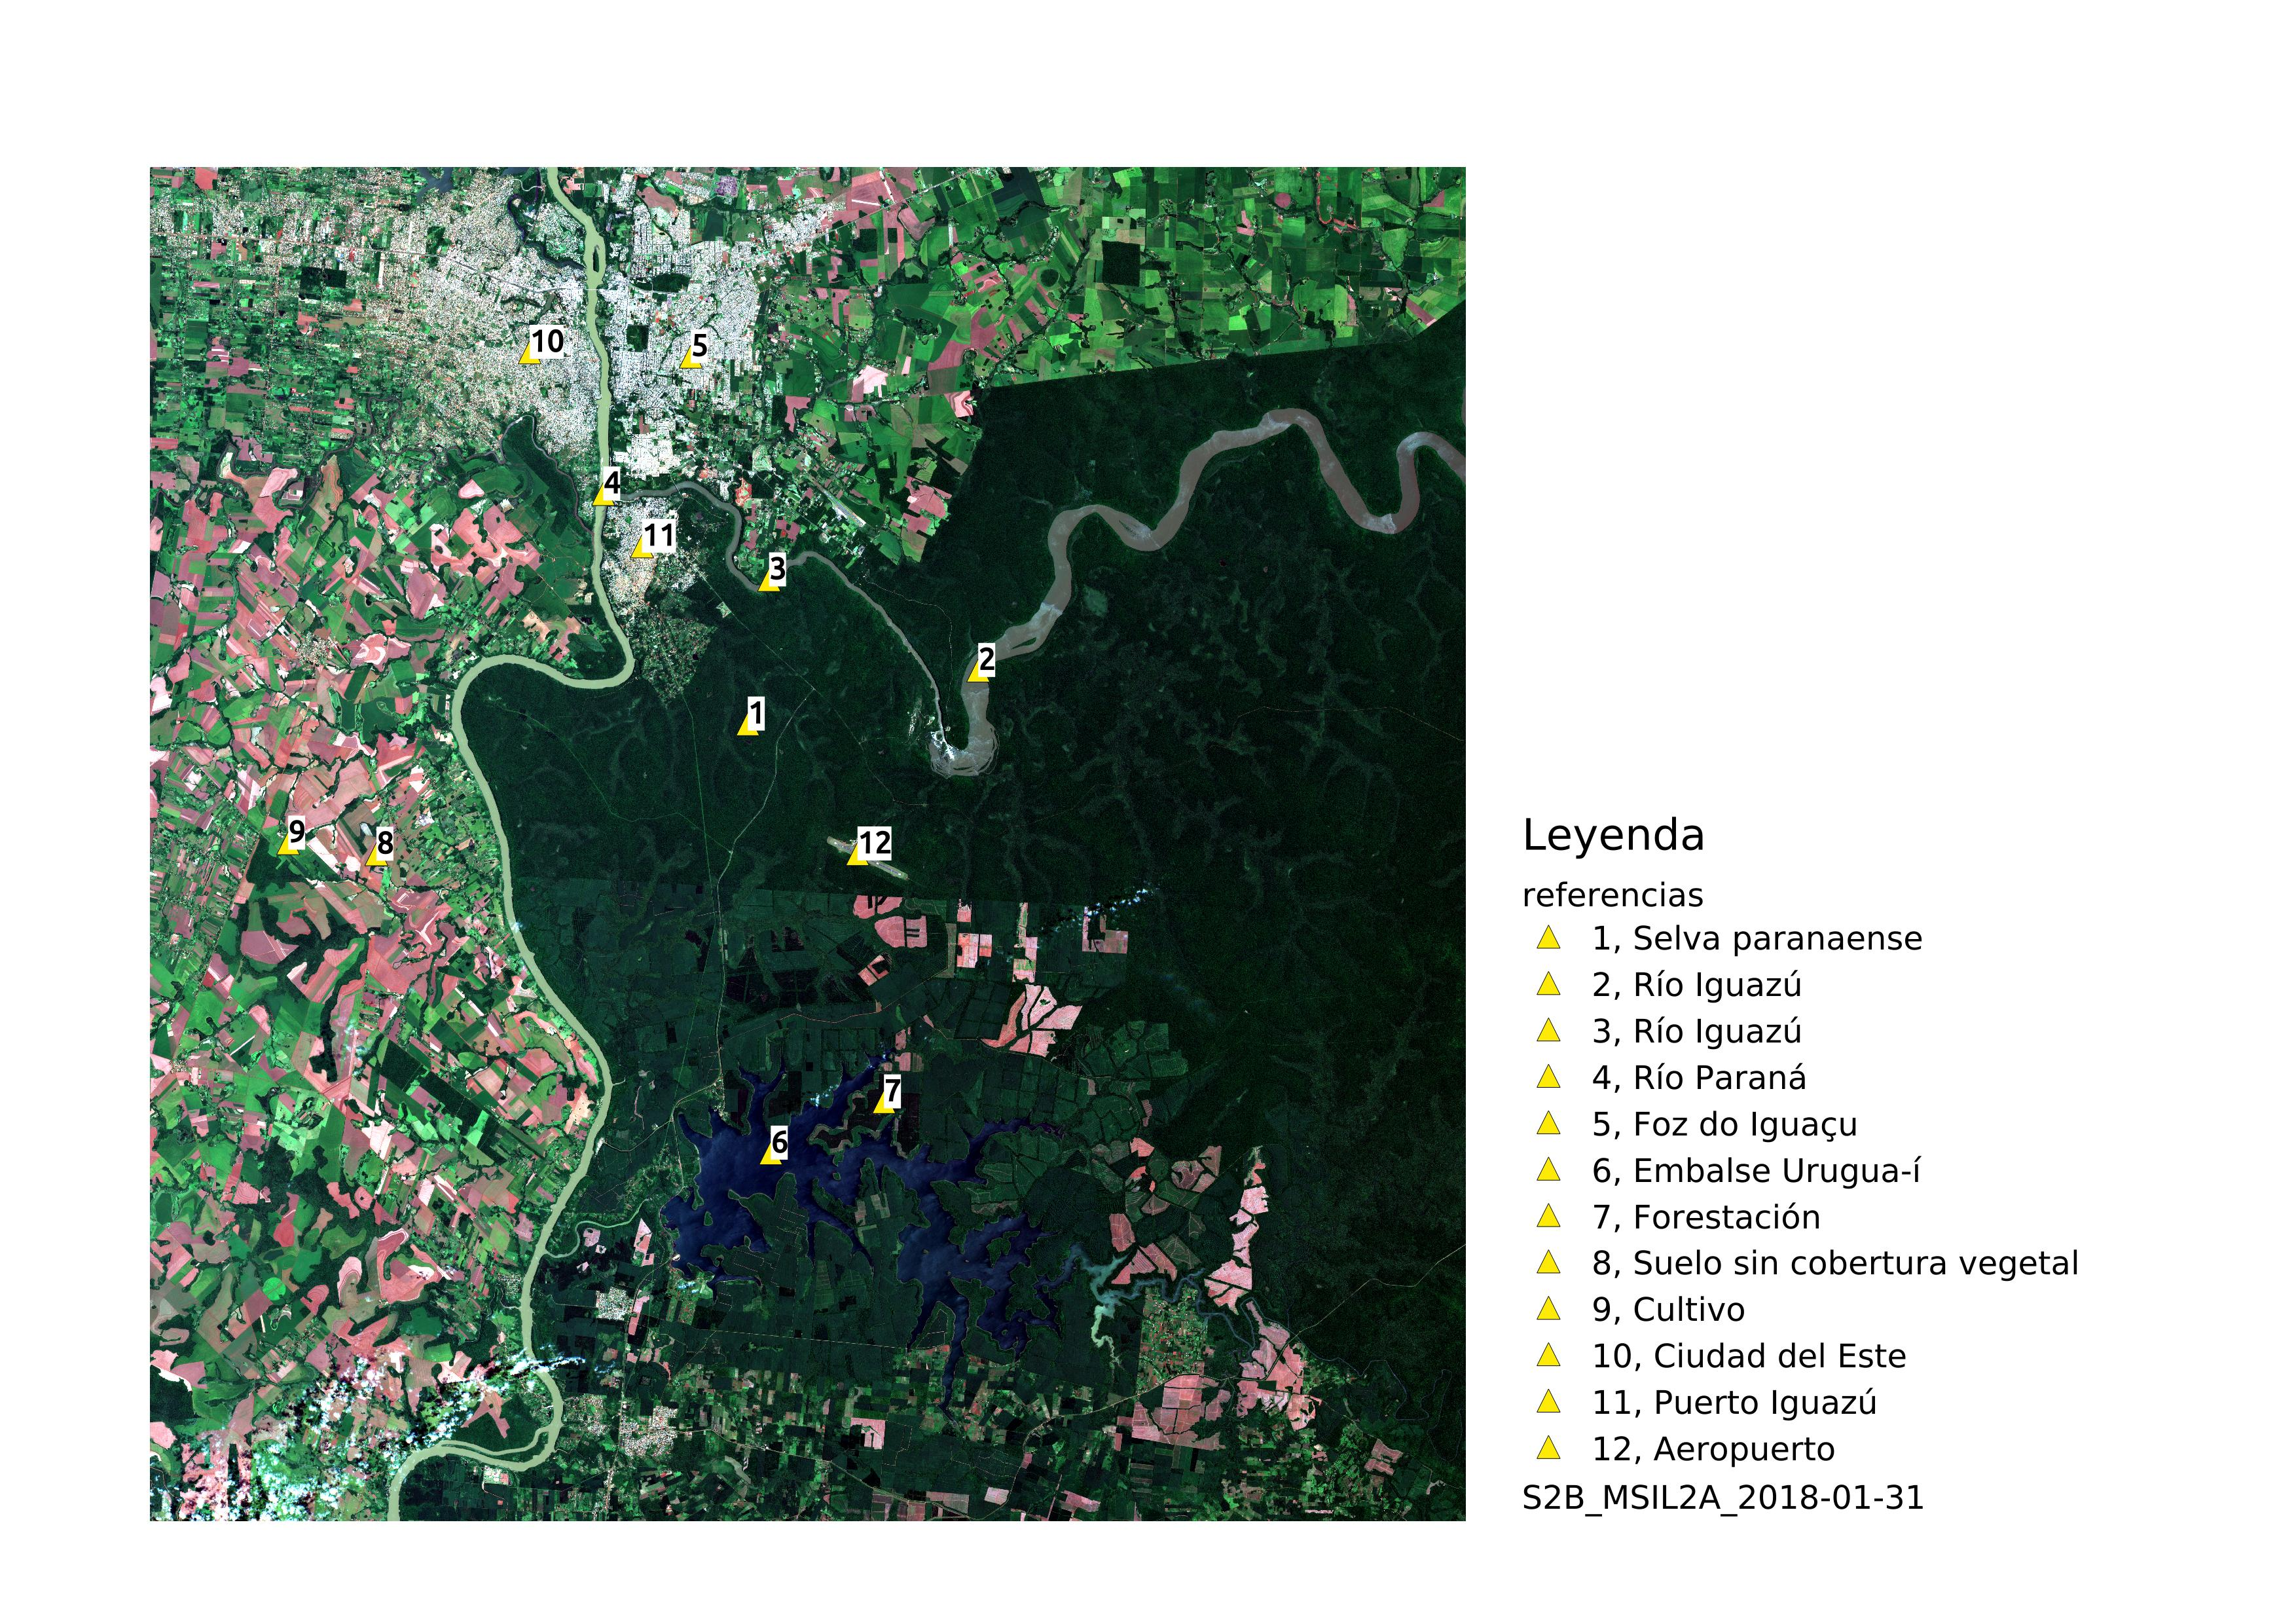
\includegraphics{fig:mapa.png}
    \caption{}
    \label{fig:mapa}
\end{figure}

\begin{itemize}
    \item La parte superior que nos permite buscar zonas en el mundo.
    \item La parte izquierda que nos permite hacer zoom en el mapa, marcar zonas de interes, realizar mediciones y agregar distintas capas como puede ser un mapa de alturas, una imagen satelital de base o un mapa politico.
    \item La parte derecha donde podemos elegir distintos productos satelitales, mostrarlos, realizar combinaciones de bandas y guardar los datos obtenidos.
\end{itemize}

En el modo mapa, busque la ciudad de Villa Carlos Paz. Podemos utilizar la herramienta medir distancias para determinar la distancia entre Córdoba Capital y Villa Carlos Paz (Figura \ref{fig:distancia}) que es de aproximadamente $30km$ en linea recta.

\begin{figure}[h!]
    \centering
    %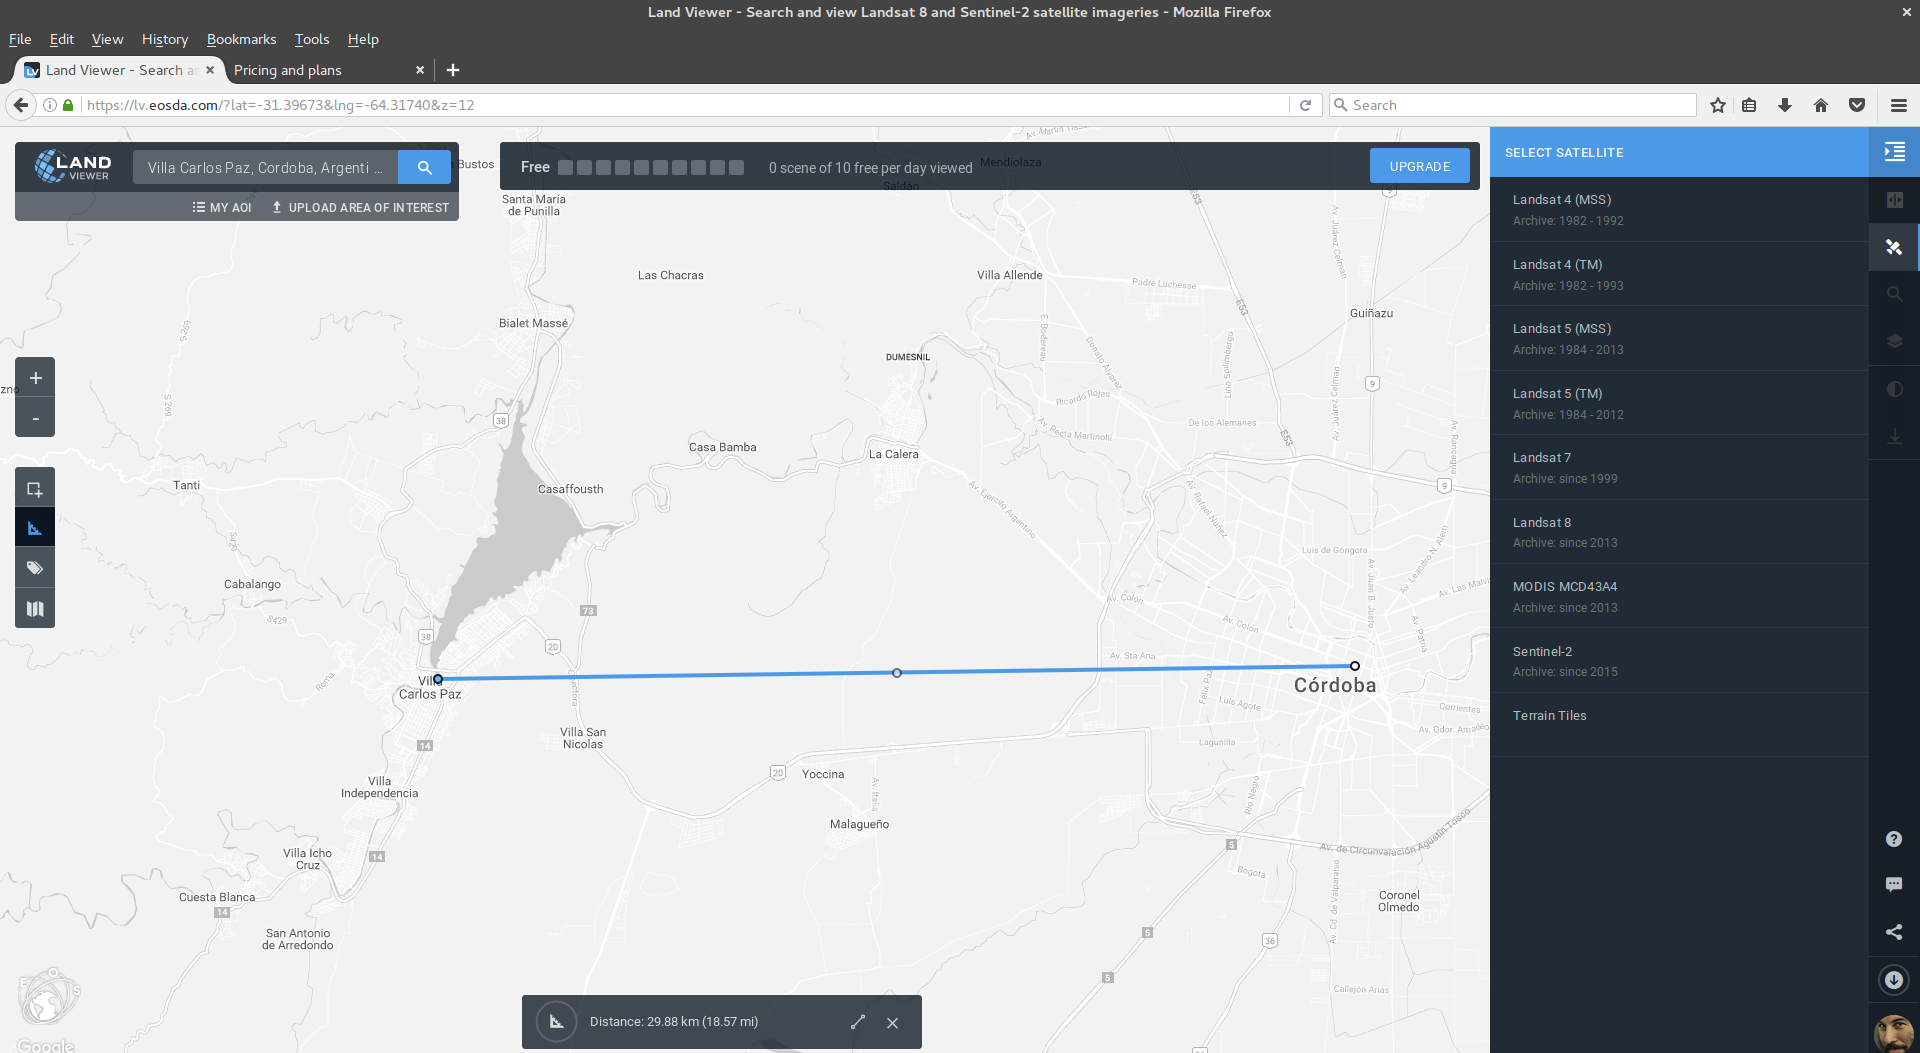
\includegraphics{fig:distancia.png}
    \caption{}
    \label{fig:distancia}
\end{figure}

Con la misma herramienta, es posible medir areas si uno cierra el camino obtenido sobre el primer punto.

\begin{que}
    ¿Cual es la superficie del Lago San Roque, que se encuentra inmediatamente al norte de Villa Carlos Paz?
\end{que}

\begin{que}
    ¿Cual es el perimetro del Lago San Roque?
\end{que}

\section{Resolución espacial y temporal} [3]
Es posible hora incorporar imágenes satelitales a nuestro mapa. Para esto comenzamos dibujando un Area de Interes (AOI) sobre la imagen que incluya la zona entre Lago San Roque y Cordoba (Figura \ref{fig:aoi}).

\begin{figure}[h!]
    \centering
    %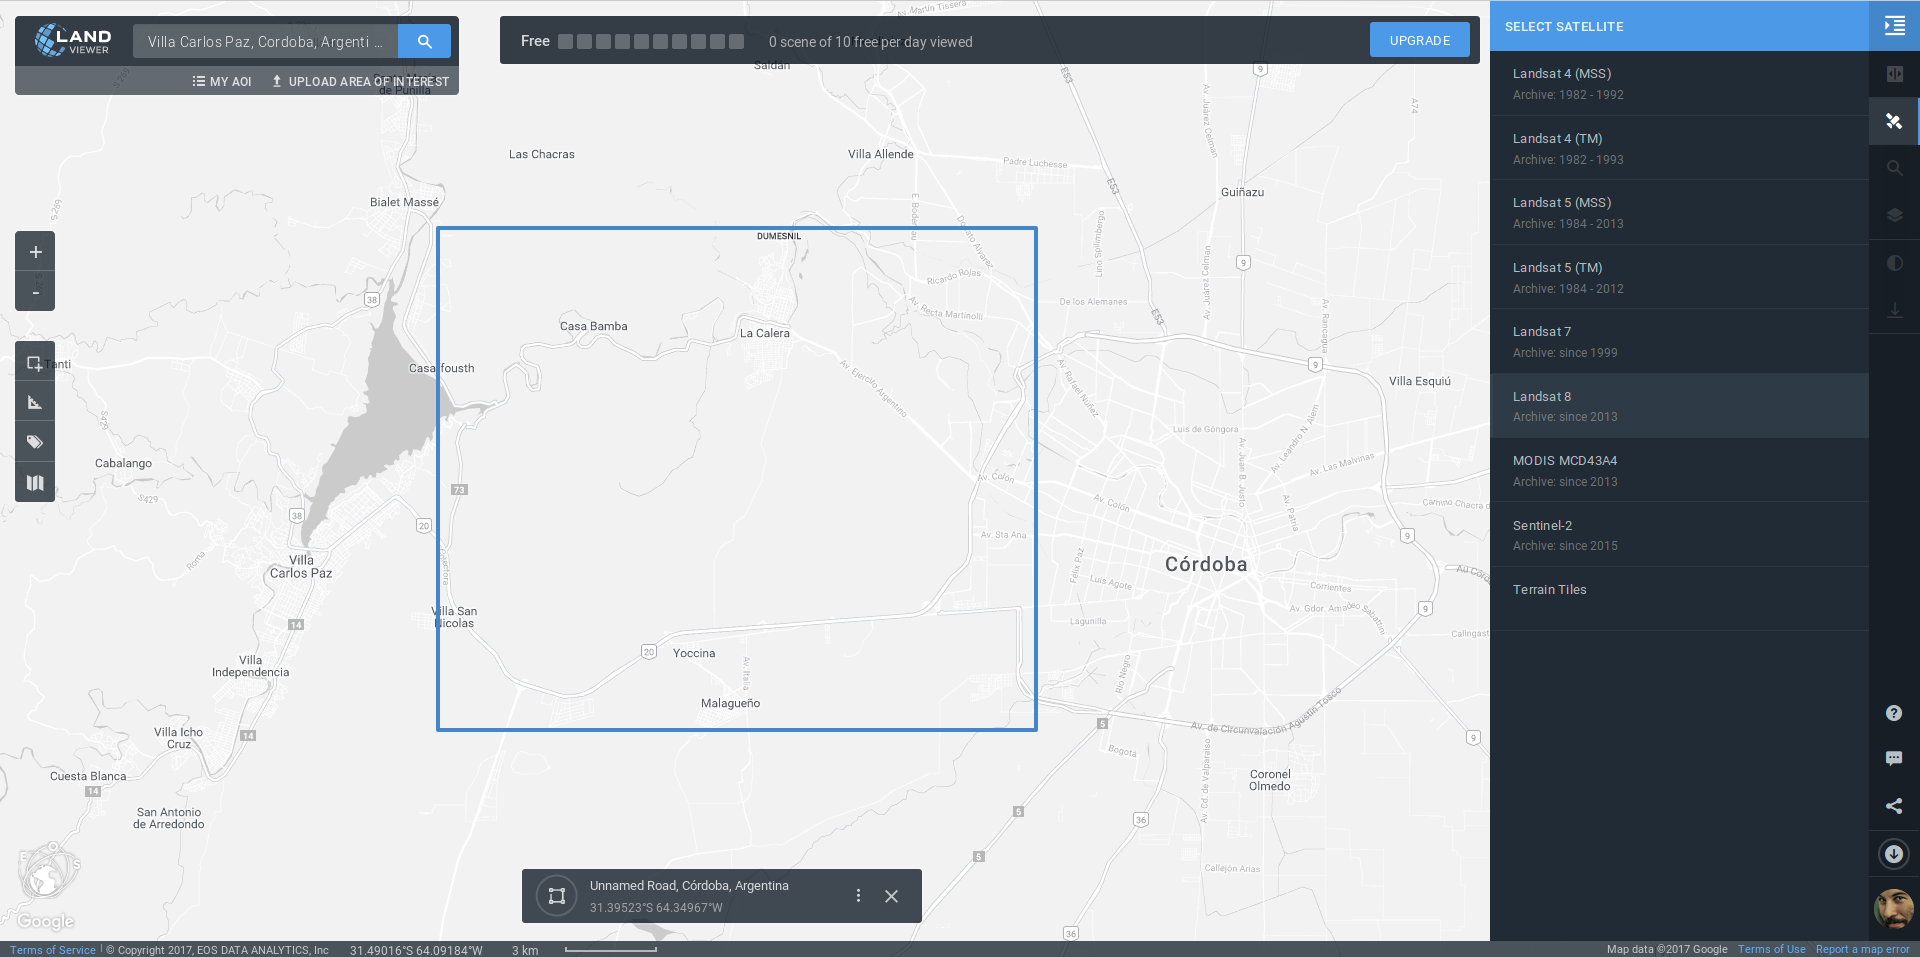
\includegraphics{fig:aoi.png}
    \caption{}
    \label{fig:aoi}
\end{figure}

Elija ahora el Satelile Landsat 8 y observe que pareceran distintas escenas a la derecha. Por defecto LandView muestra solo las escenas con cobertura nubosa de hasta un 60\% y de los últimos 3 meses. Es posible camiar hesto haciendo click en la parte superior del Scene Search.  Ponga la cobertura nubosa hasta el 100\%.

Seleccione la imagen del 2 de septiembre de 2017 y observe que esta aparecerá en la pantalla. Puede ahora moverse como hacia antes y realizar mediciones, etc.

Seleccione ahora el producto MODIS MCD43A4. Vera en este caso que la lista de imagenes es mucho más larga teniendo una imagen por día. Seleccione la imagen correspondiente al 27 de agosto de 2017.

Observe que ahora no es posible distinguir las calles de la ciudad de Córdoba como hacía con la imagen anterior. Esto muestra una relación muy importante que existe entre la resolución espacial y temporal de un producto satelital: \emph{Cuando una aumenta la otra disminuye}. Esto es normal para todos los satelites y vale hacer la observación de que ninguna es mejor o peor, solo tienen distintos usos.

\begin{que}
    ¿Cada cuantos días hay una nueva imagen Landsat 8?
\end{que}

\begin{que}
    ¿Es posible distinguir las calles de la Ciudad de Cordoba en esta imagen?
\end{que}

\section{Comparación entre fechas}
Comparemos ahora dos imagenes antes y después del incendio. Para esto sseleccione el satelite Sentinel 2 y elija la imagen del 21 de agosto de 2017. Haga luego click en \emph{Comparison slider}, cambie la fecha al año 2016 y seleccione la imagen del 23 de agosto de 2016.

Es posible elegir si la imagen se posiciona a la izquierda o la derecha eligiendolo en el botón L/R.

Puede mover ahora el slider a la izquierda y la derecha para comparar las imagenes del 2016 y 2017 (Figura \ref{fig:slider}). Elegimos comparar con el año anterior para que las imagenes correspondan a fechas similares.

\begin{figure}[h!]
    \centering
    %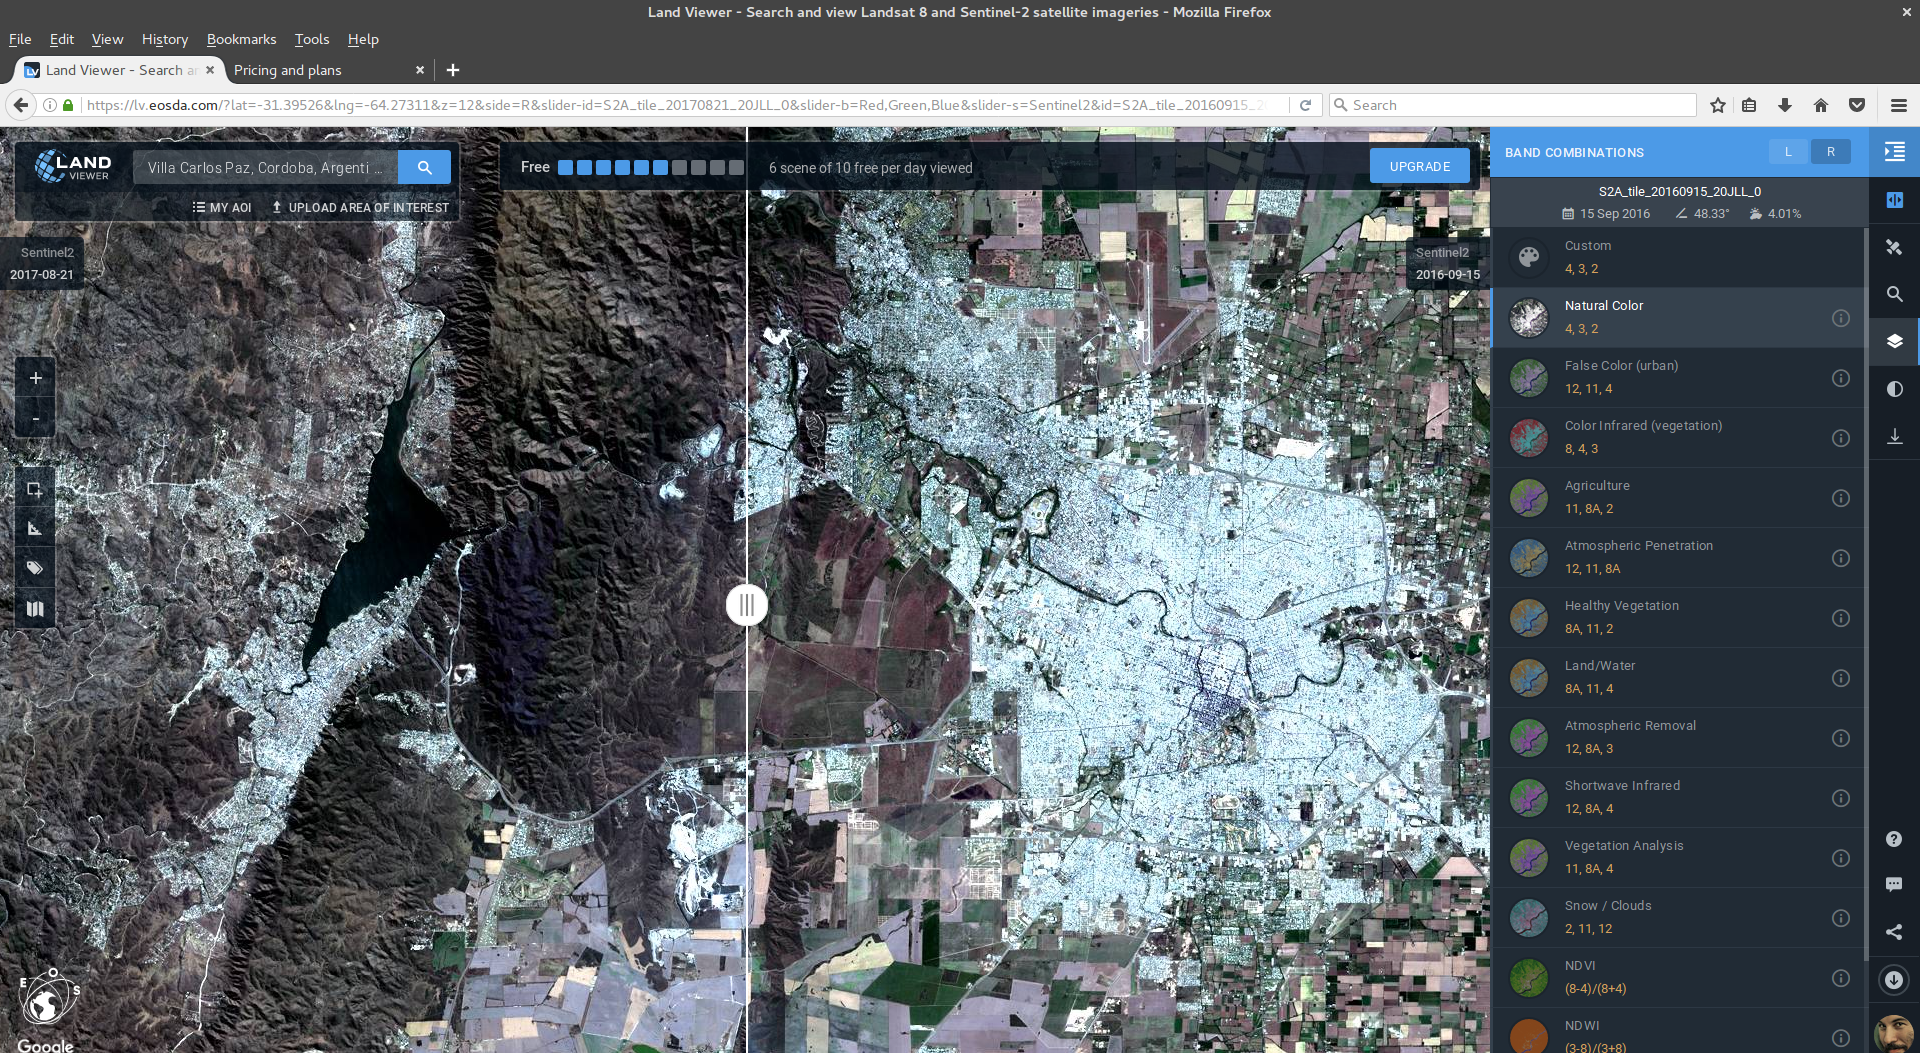
\includegraphics{fig:slider.png}
    \caption{}
    \label{fig:slider}
\end{figure}

\begin{que}
    ¿Que superficie tiene el área incendiada dentro de la imagen?
\end{que}

\begin{que}
    ¿Hay incendios en la zona durante el año 2016?
\end{que}

\section{Combinaciones de bandas} [6]
Si llego hasta acá, notará que en la combinacion de colores que estamos observando la imagen, a pesar de ser intuitiva, no permite distinguir claramente las zonas incenciadas.

Para mejorar esto es necesario entender que un satelite, como cualquier sensor, puede ser configurado para medir distintas cosas. En este caso, el satelite mide la cantidad de luz (Radiancia) que proviene de la superficie terrestre como hacen nuestros ojos. Sin embargo, a diferencia de nuestros ojos es posibles cambiar la zona del espectro electromagnetico donde medimos y como la mostramos.

Para hacer esto, realizamos las que se llaman combinaciones RGB. Mostrando de color rojo, verde y azul distinta información.

Para cambiarlas en el LandView, haga click en BAND COMBINATIONS y vera que la seleccionada es \emph{Natural Color}. Esta combinación muestra a la imagen de la forma más similar a como la veriamos nosotros.

Distintas combinaciones dde bandas permiten separar distinta información:

\begin{itemize}
    \item Color infrarred (vegetation): muestra la información sobre presencia o ausencia de vegetación en color rojo. Hace esto mostrando en rojo bandas del infrarrojo cercano y en verde y azul bandas del visible.
    \item Vegetaion analysis: muestraa la información sobre la vegetación en tonos naranjas. Hace esto mostrando en rojo información sobre la cobertura de vegetación, en verde información sobre el contenido de humedad y en azul sobre la actividad fotosintetica.
    \item False color (urban):muestra caracteristicas urbanas de nuestra coberturaa separandolas de la vegetación.
\end{itemize}

En nuestro caso particular, la combinación de bandas que mejor separa las zonas incenciadas de las no incendiadas es la \emph{Short wave infrared}. Esta combinación muestra en rojo las zonas que se incendiaron recientemente y en verde las zonas con vegetación. Eligala en el LandView y compare la imagen antes y después del incendio (Figura \ref{fig:incendio}).

\begin{figure}[h!]
    \centering
    %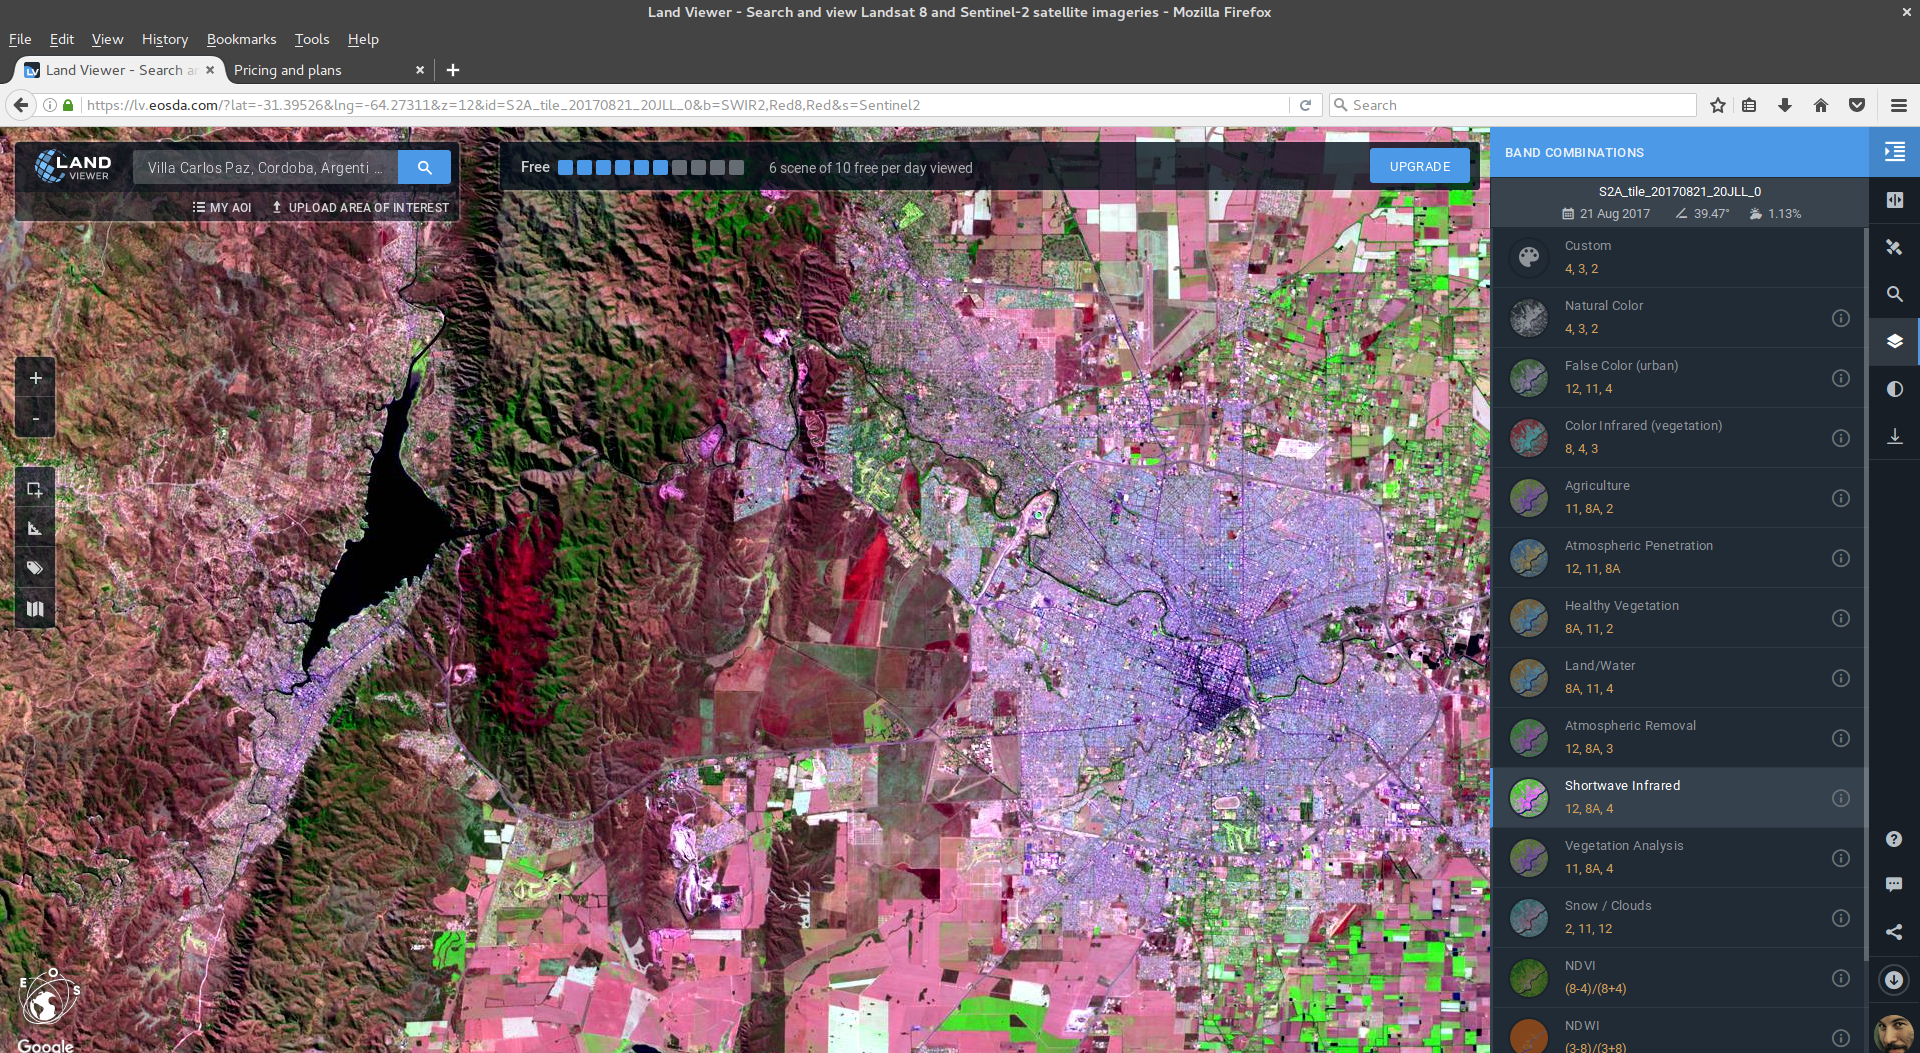
\includegraphics{fig:incendio.png}
    \caption{}
    \label{fig:incendio}
\end{figure}

Puede descargar la imagen generada haciendo click en ESCENE DOWNLOAD, eligiendo la opción de \emph{Crop by extente} y luego haciendo click en Download.

\begin{que}
    ¿Cual es la superficie incendiada al oeste del Lago San Roque?
\end{que}

\begin{que}
    Descargue un mapa de la zona donde se vea la superficie incendiada.
\end{que}

\section{Cierre}

Vimos en esta actividad como utilizar las herramientas del LandView junto con nuestro conocimiento en teledetección para interpretar distintas coberturas.

Aprendimos que hay 3 caracteristicas fundamentales de un conjunto satelite/sensor a la hora de usar productos geoespaciales

\begin{itemize}
    \item Resolucion espacial: que tan bien puedo ver algo en el suelo.
    \item Resolución temporal: cada cuanto vuelvo a tener una imagen.
    \item Resolución espectral: cuantas zonas del espectro puedo distnguir.
\end{itemize}

Este es el puntapie inicial al trabajo en teledetección donde la interpretación visual se combina con el procesamiento digital para extraer información de la vegetación. Los invitamos a que sigan de aquí en adelante.


\end{document}
